\secrel{Символьная и численная математика}\secdown

В практике любого инженера математика играет важнейшую роль. Без хорошего знания
математики, причем практически всех областей, от школьной до дифференциального
исчисления, работать в этой области практически невозможно.

Прежде всего свободное знание математики, физики и химии необходимо для чтения
любой технической литературы, особенно если вам нужно разобраться в какой-либо
прикладной области. Очень часто приходится реализовывать некоторые численные
методы вычислений, выполняющиеся в вашем устройстве в реальном времени, для
управления процессами, обработки сигналов с датчиков, принятия решений о
включении исполнительных устройств и т.п. Ну и конечно вы не сможете создать
само устройство, не понимая принципы его работы \smiley. Это конечно не
относится к различным простейшим устройствам типа таймеров или простой
автоматики, но стоимость заказов такого типа $\rightarrow 0$.

Если вы хотите поднять или восстановить свой уровень знания базовых наук (а
заодно и английского), удобно воспользоваться ресурсом
\url{https://www.khanacademy.org/}: это знаменитая on-line академия \textbf{Khan
Academy}, имеющая как набор видеолекций по базовым техническим наукам, так и
большую батарею тестов для проверки ваших знаний. Не забывайте периодически
проходить все тесты, чтобы поддерживать свои знания рабочими. Из недостатков\
--- отвратнейшая реализация на мобильных устройствах, часть тестов просто не
работает, а ввод ответов крайне неудобен из-за необходимости постоянно
пользоваться (полно)экранной клавиатурой и переключения на числовой ввод.

На русском языке ресурсов такого класса к сожалению пока не попадалось.
Кое-что есть кусочками, но по большей части только лекции в стиле <<книжкой по
башке>>, похоже навыков \emph{вводного}\ обучения в России просто не существует.
Если есть силы и желание, можете сами реализовать проект по созданию онлайн
системы базового образования \smiley.

\bigskip
В этом разделе собраны примеры проектов, требующие некоторых базовых знаний, а
также рассмотрено использование OpenSource программ для вычислений и обработки
данных.
\clearpage

\secrel{Общие сведения о компьютерной математике}

\note{Тихон Тарнавский. Maxima — максимум свободы символьных вычислений}
\note{\url{http://maxima.sourceforge.net/ru/maxima-tarnavsky-1.html}}

Для начала пару слов о том, что из себя представляют эти самые
\termdef{символьные}{символьная математика} или, как их еще называют,
\termdef{аналитические вычисления}{аналитические вычисления}, и их отличие от
численных расчетов. Компьютеры, как известно, оперируют с числами, целыми и с
плавающей запятой\note{на самом деле настоящую ``плавучку'' поддерживают только
достаточно мощные процессоры, не хуже i486dx, встраиваемые не-DSP CPU/MCU
аппаратно работают только с целыми числами: $\pm 127$, $\pm (2^{16}-1)$ и $\pm
(2^{32}-1)$\ в зависимости от разрядности ядра 8- 16- или 32-бит}. К примеру,
решения уравнения $x^{2} = 2x + 1$ можно получить как -0.41421356 и 2.41421356,
а $3x = 1$\ --- как 0.33333333. А ведь хотелось бы увидеть не приближенную
цифровую запись, а точную величину, т. е. $1\pm\sqrt{2}$ в первом случае и $1/3$
во втором. С этого простейшего примера и начинается разница между численными и
символьными вычислениями.

Но кроме этого, есть еще задачи, которые вообще невозможно решить численно или
наоборот аналитически.

Например, параметрические уравнения, где в виде решения нужно выразить
неизвестное через параметр; или нахождение производной от функции; да
практически любую достаточно общую задачу можно решить только в символьном виде.

Наоборот, для многих задач не существует точного аналитического решения, и
приходится применять \termdef{численные методы}{численные методы}\ их решения.

В некоторых случаях нужно получение простого и быстрого \termdef{приближенного
решения}{приближенное решение}\ --- это может понадобится в системах управления,
когда микроконтроллер не успевает за управляемым процессом, если пытается
получить точное численное решение. При обработке сигналов например не требуется
точное решение, достаточно результата, получаемого численными методами.

Для решения аналитических задач давно появились компьютерные программы,
оперирующие любыми математическими объектами, от чисел любого типа, векторов и
матриц до тензоров, от функций до интегро-дифференциальных уравнений и т.д.\
--- они имеют общее название \termdef{CAS}{CAS}: [C]omputer [A]lgebra [S]ystem.

Среди математического ПО для аналитических (символьных) вычислений наиболее
известны коммерческие CAS-пакеты \prog{Maple}, \prog{Mathematica} и
\prog{MathCAD}. Для символьных вычислений предназначен пакет \prog{MatLab}.
Это очень мощные и \emph{очень дорогие} инструменты для ученых и инженеров,
позволяющие автоматизировать наиболее рутинную и требующую повышенного внимания
часть работы, оперируя при этом аналитической записью данных и терминами
предметной области, т.е. почти математическими формулами.

Такие программы можно назвать \emph{средой математического программирования}, с
той разницей, что в качестве элементов языка программирования выступают
привычные человеку математические обозначения.

Для преподавателей, аспирантов, и студентов предоставляются академические более
дешевые лицензии, но для хоббитов и коммерческого применения требуется покупка
полной лицензии, имеющей зачастую космическую стоимость. Неплохим вариантом
может послужить использование бесплатного и свободного OpenSource программного
обеспечения, описанного далее\ --- пакетов \prog{Maxima}\  и \prog{Octave}.

С другой стороны, основное направление, кроме научных разработок, где такие
программы востребованы\ --- высшее образование; а использование для учебных нужд
именно свободного ПО\ --- реальная возможность и для ВУЗа, и для студентов и
преподавателей иметь в своем распоряжении легальные копии такого ПО без больших,
и даже каких-либо денежных затрат.

\secrel{Пакет Octave}\secdown

\prog{Octave}\ -- пакет CAS для численных вычислений.

\bigskip\noindent
\begin{tabular}{p{0.25\textwidth} p{0.75\textwidth}}
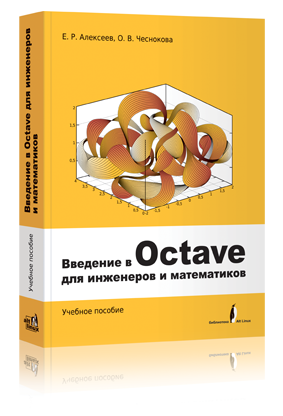
\includegraphics[height=0.45\textheight]{math/octave/BookOctave.png}
&
\parbox[b]{0.7\textwidth}{
Е.Р. Алексеев, О.В. Чеснокова\\
\textbf{Введение в Octave для инженеров и математиков}\\
\url{http://www.altlinux.org/Books:Octave}
}
\\
\end{tabular}

\secup

\secrel{Пакет Maxima}\secdown

\prog{Maxima}\ -- пакет CAS символьной математики.

\bigskip\noindent
\begin{tabular}{p{0.25\textwidth} p{0.75\textwidth}}
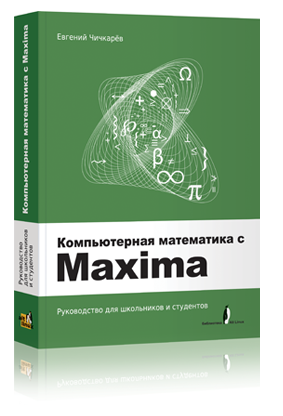
\includegraphics[height=0.45\textheight]{math/maxima/BookMaxima.png}
&
\parbox[b]{0.7\textwidth}{
Евгений Чичкарёв\\
\textbf{Компьютерная математика с Maxima. Руководство для школьников и
студентов}\\
\url{http://www.altlinux.org/Books:Maxima}\\
}
\\
\end{tabular}

\bigskip
Дополнительная документация:
\url{http://maxima.sourceforge.net/ru/documentation.html}

\bigskip\noindent
\href{https://drive.google.com/file/d/0B0u4WeMjO894M01wZmNkSW9GRHM/view?usp=sharing}{PDF}\
для книги Ильина В.А., Силаев П.К. Система аналитических вычислений Maxima для
физиков-теоретиков\ \cite{maxphis}\ получена из файла \file{.ps}\ с помощью
сервиса \url{http://ps2pdf.com/convert.htm}.

\secrel{Установка Maxima под \win}

\menu{\winr>\url{http://maxima.sourceforge.net/ru/}>Загрузка}

\menu{Maxima-Windows>\file{5.34.1-Windows}>\file{maxima-5.34.1.exe}}

\menu{\file{maxima-5.34.1.exe}>Установка>Язык>\textbf{English}>OK>Next}

\menu{License>I accept>Next>}

\menu{Install folder>по умолчанию>Next}

\menu{Components>\uncheckbox\ Language packs>Next>Next}

\menu{\checkbox\ wxMaxima>\uncheckbox\ XMaxima>Next>Install>Next>Finish}

\menu{\winstart>Maxima-5.34.1>wxMaxima>\rms>Закрепить в панели задач}

\secup


\secrel{Параллельные вычисления}\secdown
\secrel{Многоядерные архитектуры с разделяемой памятью} 
\secrel{Кластер архитектуры Beowulf}
\secrel{Вычисления на GPU}
\secrel{Средства параллелизации \cpp}
\secrel{BLAS/LAPACK/MPI/ScalaPack}
\secrel{Средства измерения производительности}
\secup


\secup
